\documentclass{article} 

\usepackage{geometry}
\usepackage{indentfirst}
\usepackage{fancyhdr}
\usepackage{caption}
\usepackage{graphicx}
\usepackage{enumitem}
\usepackage{hyperref}
\usepackage{tabularx}

\pagestyle{fancy}
\geometry{a4paper, margin=1in}
\captionsetup{labelformat=empty}
\graphicspath{ {../../assets/SRS_images/} }\begin{document}

\title{Software Requirements Specification for Viper Rocks!}
\author{Version 1.0.0}
\date{Group 2}

\maketitle
\tableofcontents
\newpage

\fancyhf{}
\fancyhead[C]{Software Requirements Specification}
\fancyfoot[C]{\thepage}

\begin{table}[h!]
\centering
\caption{\textbf{Revision History}}
\begin{tabularx}{\textwidth}{|c|c|X|c|}
\hline
\textbf{Name} & \textbf{Date} & \textbf{Reasons for Changes} & \textbf{Version} \\
\hline
Tony Lau & 2/20/25 & First Draft & 1.0.0 \\
\hline

\hline

\hline

\hline
\end{tabularx}
\end{table}

\section{Introduction}
The VIPER Rocks! project is a thrilling initiative that empowers citizen scientists, both amateur and expert, to participate in unraveling the mysteries of lunar geology. This project leverages the power of citizen science to map and classify lunar rocks encountered during VIPER's historic exploration of the Moon's South Pole.

Ultimately, VIPER Rocks! plays a vital role in establishing a sustainable presence on the Moon. By mapping and analyzing the distribution of ice and other resources near the Moon's South Pole, VIPER Rocks! paves the way for future missions to Mars and beyond.

This Software Requirements Specification (SRS) serves as a comprehensive guide to the technical aspects of the VIPER Rocks! project. It outlines the requirements, features, and functionality of the software that will enable citizen scientists to contribute to lunar geology research. The document also contains the project's objectives, user interfaces, technical approach, and testing strategies to ensure the successful development of VIPER Rocks!

\subsection{Purpose}
This SRS is intended for various stakeholders involved in the VIPER Rocks! project, including software developers, project managers, data analysts, beta testers, and anyone interested in the technical details of the application. It provides a reference for understanding the project's scope, technical requirements, and functionality. It is organized for various types of readers, and each type of reader may interpret this document differently:

\subsection{Internal Audience and Reading Suggestions}
Our intended audience includes: 
\begin{itemize}
	\item Software Developers
	\item Project Managers
	\item Data Analysts
\end{itemize}

\subsection{Product Scope}

\subsubsection{Product}
This product is the "VIPER Rocks!" citizen science website

\subsubsection{Description}
The VIPER Rocks! software will enable citizen scientists to actively participate in mapping and classifying lunar rocks encountered during NASA's VIPER mission. It will facilitate the scientific analysis of lunar rock populations and enhance our understanding of lunar geology. The software will allow users to measure rock size and classify rock shape, on both mobile and desktop displays.

\subsubsection{Objectives}
The software aims to enhance the science return of the VIPER mission and engage the public in lunar exploration. The objectives include creating this citizen science platform and improving our understanding of lunar rock populations.

\subsection{Definitions, Acronyms, and Abbreviations}
\begin{itemize}
	\item VIPER - Volatiles Investigating Polar Exploration Rover
	\item UI - User Interface
\end{itemize}

\section{External Interface Requirements}

\subsection{User Interfaces}
USDS: \href{https://designsystem.digital.gov/}{https://designsystem.digital.gov/} \\
NASAWDS: \href{https://github.com/bruffridge/nasawds}{https://github.com/bruffridge/nasawds} \\
We will be sticking with a dark and blue color scheme. Below are the components we will make use of: \\
Buttons: \\
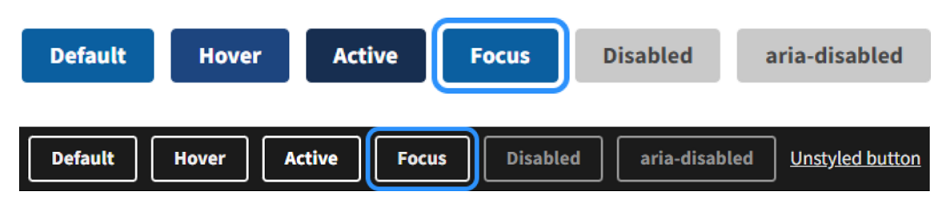
\includegraphics{buttons} \\
Headers, Footers, Radio Buttons: \\
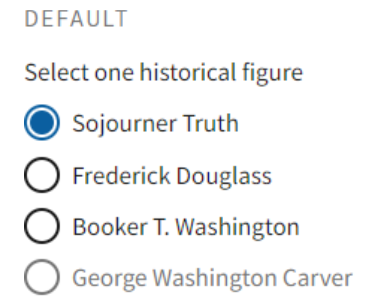
\includegraphics{headers} \\
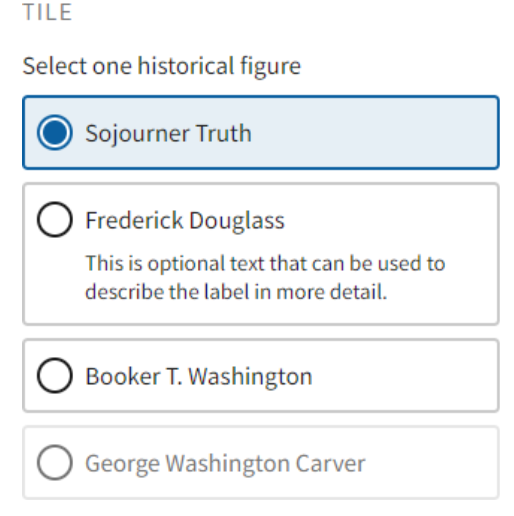
\includegraphics{footers} \\
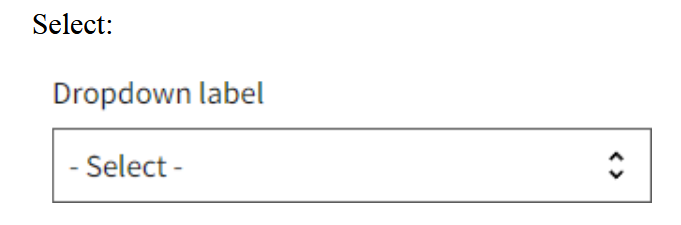
\includegraphics{radiobuttons} \\
Tags: \\
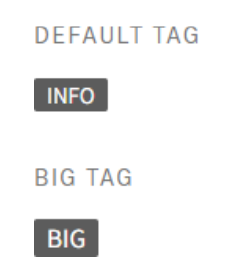
\includegraphics{tags} \\
Text Inputs: \\
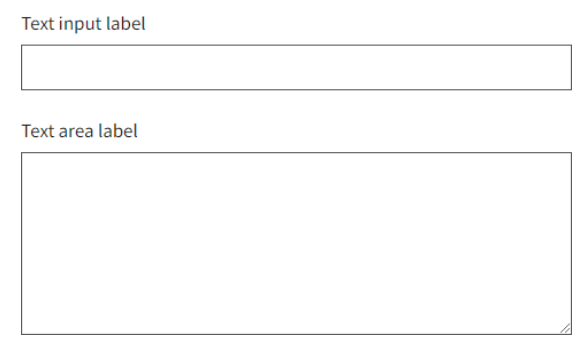
\includegraphics{text_inputs} \\
Typefaces: Source Sans Pro, Public Sans, Roboto Mono, Merriweather

The following images are draft mockups of the landing and scouting pages (not all mockups are finished yet): \\
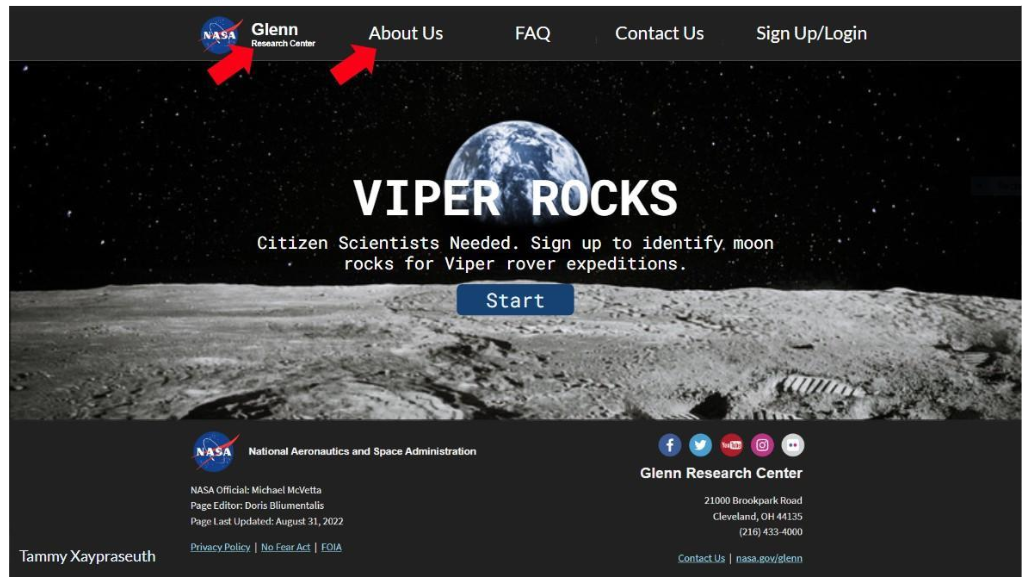
\includegraphics{landing_page_1}
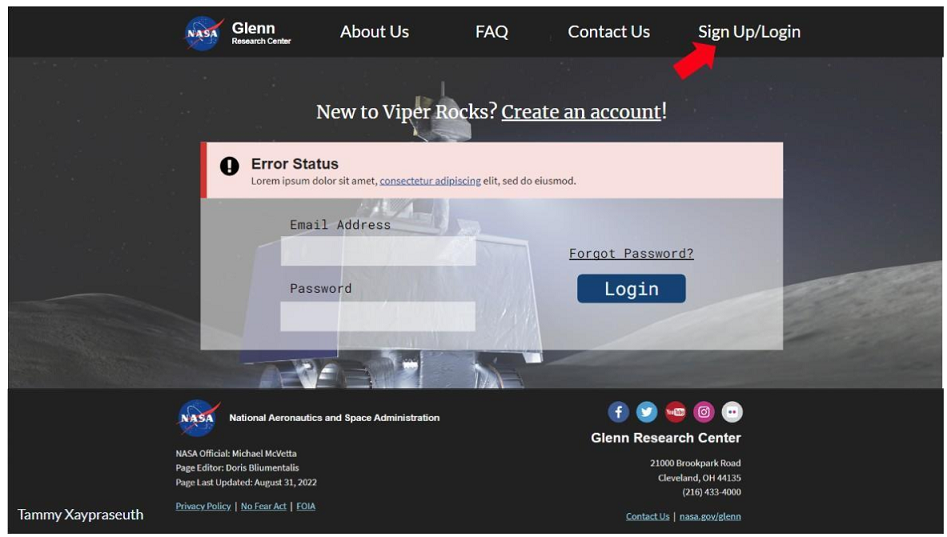
\includegraphics{landing_page_4}
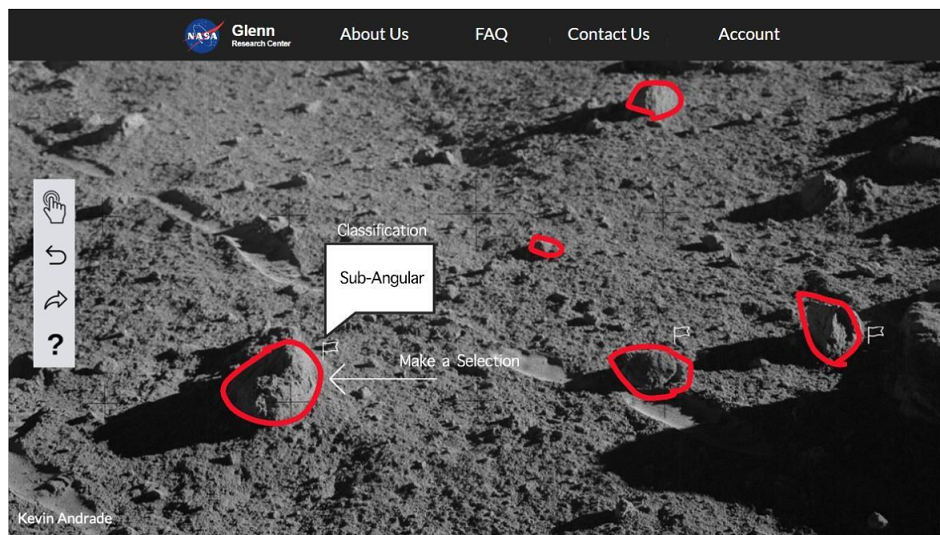
\includegraphics{scouting_page}
We will be adhering closely to the Americans with Disabilities Act to make it accessible to as many users as possible. We will also look to and reference the USWDS and NASA Guidelines for guidance on accessible designs.

\subsection{Hardware Interfaces}
The following are different input systems that will be kept in mind while developing this web application. Users will need a mobile device or personal computer. If they have a personal computer, they will require a mouse and keyboard or a trackpad.
\subsection{Software Interfaces}
The following are software interfaces that will be used for this product
\begin{itemize}
	\item React
	\item MySQL
	\item MongoDB
	\item Javascript
	\item Node.js
\end{itemize}
\subsection{Communications Interfaces}
Users will need an email if they choose to contact the team. The team’s emails are listed on the website for anybody to contact.

\section{Legal and Ethical Considerations}
The various legal and ethical considerations that must be addressed to ensure the protection of users and the responsible conduct of scientific research include:

\textbf{Privacy}:
\begin{itemize}
	\item The project must clearly inform users about the types of data collected through the application and how it will be used.
	\item User consent must be obtained explicitly before collecting any personal information.
\end{itemize}
\textbf{Security}: 
\begin{itemize}
	\item The security of the user’s data must be maintained. Methods will be implemented to ensure it stays secure and private.
\end{itemize}

\section{Appendix A: Glossary}
\begin{itemize}
	\item LUNAR - Lunar Uplink for Navigation and Analysis of Reconnaissance
\end{itemize}


\end{document}